\section{Esponenziale}
Modella il tempo di attesa tra eventi in un processo di Poisson di intensità $\lambda>0$ (ad esempio, il tempo fino al prossimo arrivo).

\[
\mathcal{E}(\lambda)
\]

\begin{figure}[H]
\centering

\begin{minipage}{0.45\textwidth}
\centering
\begin{tikzpicture}
\begin{axis}[
    axis lines = middle,
    ylabel = {$f(x)$},
    xlabel = {$x$},
    width = 0.90\textwidth,
    height = 0.90\textwidth,
    ymin = 0, ymax = 0.55,
    xmin = -1, xmax = 26
]

% --- Exponential(lambda=0.2) ---
\addplot[
    black,
    thick,
    domain=0:26,
    samples=300
]
{0.2*exp(-0.2*x)};


% --- Exponential(lambda=0.5) ---
\addplot[
    gray!60,
    thick,
    domain=0:26,
    samples=300
]
{0.5*exp(-0.5*x)};


\end{axis}
\end{tikzpicture}
\end{minipage}
\hfill
\begin{minipage}{0.45\textwidth}
\centering

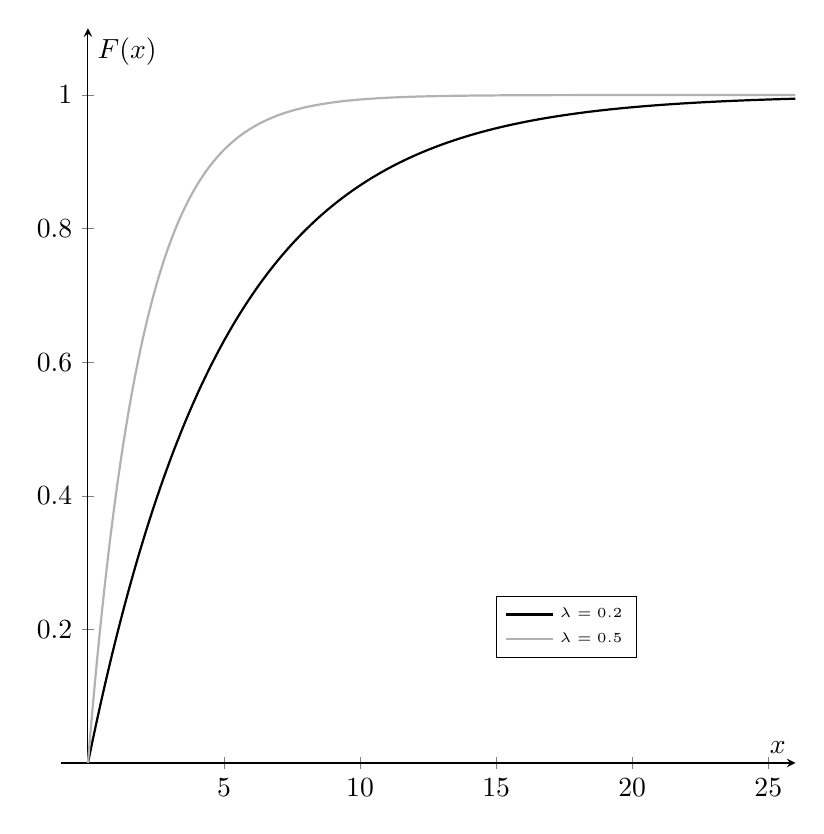
\begin{tikzpicture}
\begin{axis}[
    axis lines = middle,
    ylabel = {$F(x)$},
    xlabel = {$x$},
    width = 0.90\textwidth,
    height = 0.90\textwidth,
    ymin = 0, ymax = 1.1,
    xmin = -1, xmax = 26,
    legend style={at={(axis cs: 15,0.25)}, anchor=north west, font=\tiny},
    legend cell align=left,
]

% --- CDF Exponential(lambda=0.2) ---
\addplot[
    black,
    thick,
    domain=0:26,
    samples=300
]
{1 - exp(-0.2*x)};
\addlegendentry{$\lambda=0.2$}

% --- CDF Exponential(lambda=0.5) ---
\addplot[
    gray!60,
    thick,
    domain=0:26,
    samples=300
]
{1 - exp(-0.5*x)};
\addlegendentry{$\lambda=0.5$}

\end{axis}
\end{tikzpicture}

\end{minipage}

\end{figure}

\bigskip
\begin{table}[H]
\centering
\renewcommand{\arraystretch}{2}
\begin{tabular}{@{}ll@{}}
\toprule
\textbf{Supporto} 
& $[0,+\infty)\subset\mathbb{R}$ \\

\midrule

\textbf{Funzione di Densità} 
& $f(x)=\lambda e^{-\lambda x}\,\mathbb{I}_{(0, +\infty)}(x)$\\

\midrule

\textbf{Funzione di Ripartizione}
& $F(x)=\bigl(1-e^{-\lambda x}\bigl)\,\mathbb{I}_{(0, +\infty)}(x)$ \\

\midrule

\textbf{Valore atteso} 
& $\mathbb{E}[X]=\dfrac{1}{\lambda}$ \\

\midrule

\textbf{Varianza}
& $Var(X)=\dfrac{1}{\lambda^2}$ \\

\midrule

\textbf{Funzione caratteristica}
& $\varphi_X(u)=\dfrac{\lambda}{\lambda-iu}$ \\

\bottomrule
\end{tabular}
\end{table}

\noindent La distribuzione esponenziale è l’unica distribuzione continua non degenere a possedere la \emph{proprietà di assenza di memoria}. 
Essa afferma che, per ogni $s,t \ge 0$,
\[
\mathbb{P}(X > s+t \mid X > s) = \mathbb{P}(X > t).
\]

Dal punto di vista probabilistico, questa relazione implica che il tempo di attesa residuo non dipende dal tempo già trascorso: il processo “riparte da zero” in ogni istante, indipendentemente dalla sua storia passata. Questo la rende perfetta per modellizzare il tempo di vita di oggetti che non
invecchiano.